\section{Teoremi generali}
Questa sezione vuole raccogliere alcuni teoremi importanti che però non appartengono a nessuna sezione precedente in particolare in quanto richiedono l'uso di molti argomenti presi da sezioni differenti. Ho quindi congegnato che era meglio dedicare loro una sezione a parte, sperando che il mio intento di organizzazione possa essere apprezzato da quelli che leggeranno.

\subsection{Teorema degli zeri}
Il teorema degli zeri è estremamente importante in analisi. In pratica afferma che se una funzione è continua e ha un punto in cui è positiva (quindi è sopra l'asse delle ascisse) e un punto in cui è negativa (quindi è sotto l'asse delle ascisse), per forza tra quei due punti ce ne sarà un terzo in cui la funzione tocca l'asse delle ascisse. È abbastanza facile verificare che è vero in quanto se si vuol tracciare una linea continua che in punto è sopra l'asse delle ascisse e in un altro è sotto, per forza si è costretti ad intersecare tale asse.
\begin{figure}[h]
    \centering
    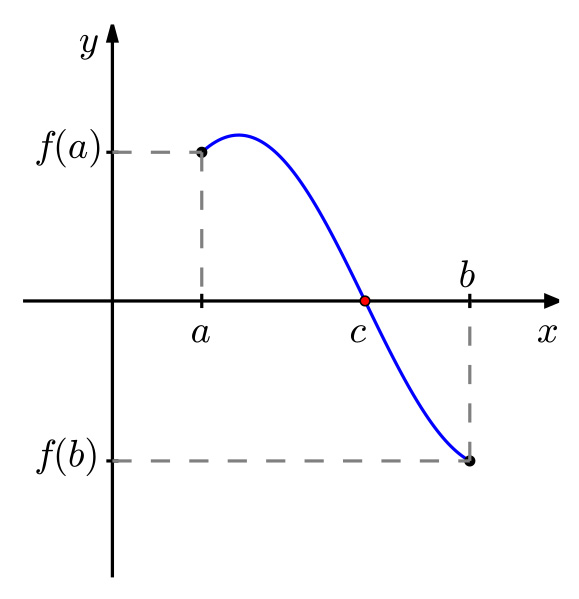
\includegraphics[width=180px]{../img/TeoremaZeri.jpg}
    \caption{Rappresentazione grafica del teorema degli zeri}
\end{figure}
Per dimostrare questo teorema abbiamo però bisogno di due lemmi preliminari:

\mlem{
Data una successione $(a_n)_n \subseteq \mathbb{R}$ , se 
\begin{equation*}
    \forall n, a_n < 0 \implies \lim _{x \to +\infty} a_n = l \in R \; \land \; l \leq 0
\end{equation*}
Si noti che questo lemma vale anche per il caso in cui $\forall n, a_n > 0$, che implica $l \geq 0$. Dimostriamo ora il lemma\footnote{La seguente dimostrazione è stata fatta dal prof in maniera imbarazzante, quindi la esplicito secondo la logica classica per renderla più formale}. Dobbiamo provare che:
\begin{equation*}
    \forall n, a_n < 0 \implies \lim _{x \to +\infty} a_n = l \leq 0
\end{equation*}
Fisso $n$ numero t.c $\forall n, a_n < 0$ (H) per dimostrare:
\begin{equation*}
    \lim _{x \to +\infty} a_n = l \leq 0
\end{equation*}
Per assurdo assumiamo\footnote{Abbiamo usato il potere sconfinato della RAA (Coen approves)} $l > 0$ (H2) e riduciamoci a dimostrare il falso. Grazie alla definizione di limite possiamo riscrivere il limite nel seguente modo:
\begin{equation*}
    \forall \epsilon > 0, \exists \overline{n} \in \mathbb{N} : \forall n \geq \overline{n} \implies |q_n - l| < \epsilon
\end{equation*}
Se espandiamo $|q_n - l| < \epsilon$ ci troviamo con:
\begin{equation*}
    l - \epsilon < a_n < l + \epsilon
\end{equation*}
Ed essendo che questa condizione delle valere $\forall \epsilon > 0$, scegliamo $\epsilon = \dfrac{l}{2}$. Quindi deve valere che:
\begin{equation*}
    a_n > l - \epsilon = l - \dfrac{l}{2} = \dfrac{l}{2}
\end{equation*}
Per (H2) $\dfrac{l}{2} > 0$ ma per (H) $\forall n, a_n < 0$. ASSURDO in quanto $a_n$ non può contemporaneamente essere maggiore di $0$ e minore di $0$.\\

\hfill Qed.
}

\mlem{
Data una funzione $f: A \to \mathbb{R}$, un punto $x_0 \in A \cap \mathcal{D}(A)$ e inoltre $f$ deve essere continua in $x_0$:
\begin{equation*}
    \forall (a_n)_n \subseteq A : a_n \to x_0 \implies f(a_n) \xrightarrow[n \to + \infty]{} f(x_0)
\end{equation*}
}

\thm {
\begin{equation*}
f:[a,b] \to \mathbb{R}\;\; \text{continua, }\; f(a) \cdot f(b) < 0 \implies \exists c \in ]a,b[ : f(c) = 0
\end{equation*}
}
Un paio di osservazioni utili sul teorema:
\begin{itemize}
    \item La continuità di $f$ è fondamentale in quanto se non lo fosse il teorema non potrebbe valere. Si consideri infatti il caso di una funzione definita a tratti nel seguente modo:
    \begin{equation*}
        f(x) =
        \begin{cases*}
            -1 \qquad (0 \leq x \leq 2)\\
            1   \qquad \;\;\;(2 < x \leq 4)
        \end{cases*}
    \end{equation*}
    Quest'ultima rispetta tutte le specifiche del teorema ($f(0) \cdot f(4) < 0$) tranne la continuità (non è infatti continua in $x = 2$). Se si osserva il grafico (Figura: \ref{Figura_TeoraZeri}) si nota subito che questa funzione non ammette nessun punto in cui si annulla come vorrebbe il teorema degli zeri.
    \begin{figure}[h]
        \centering
        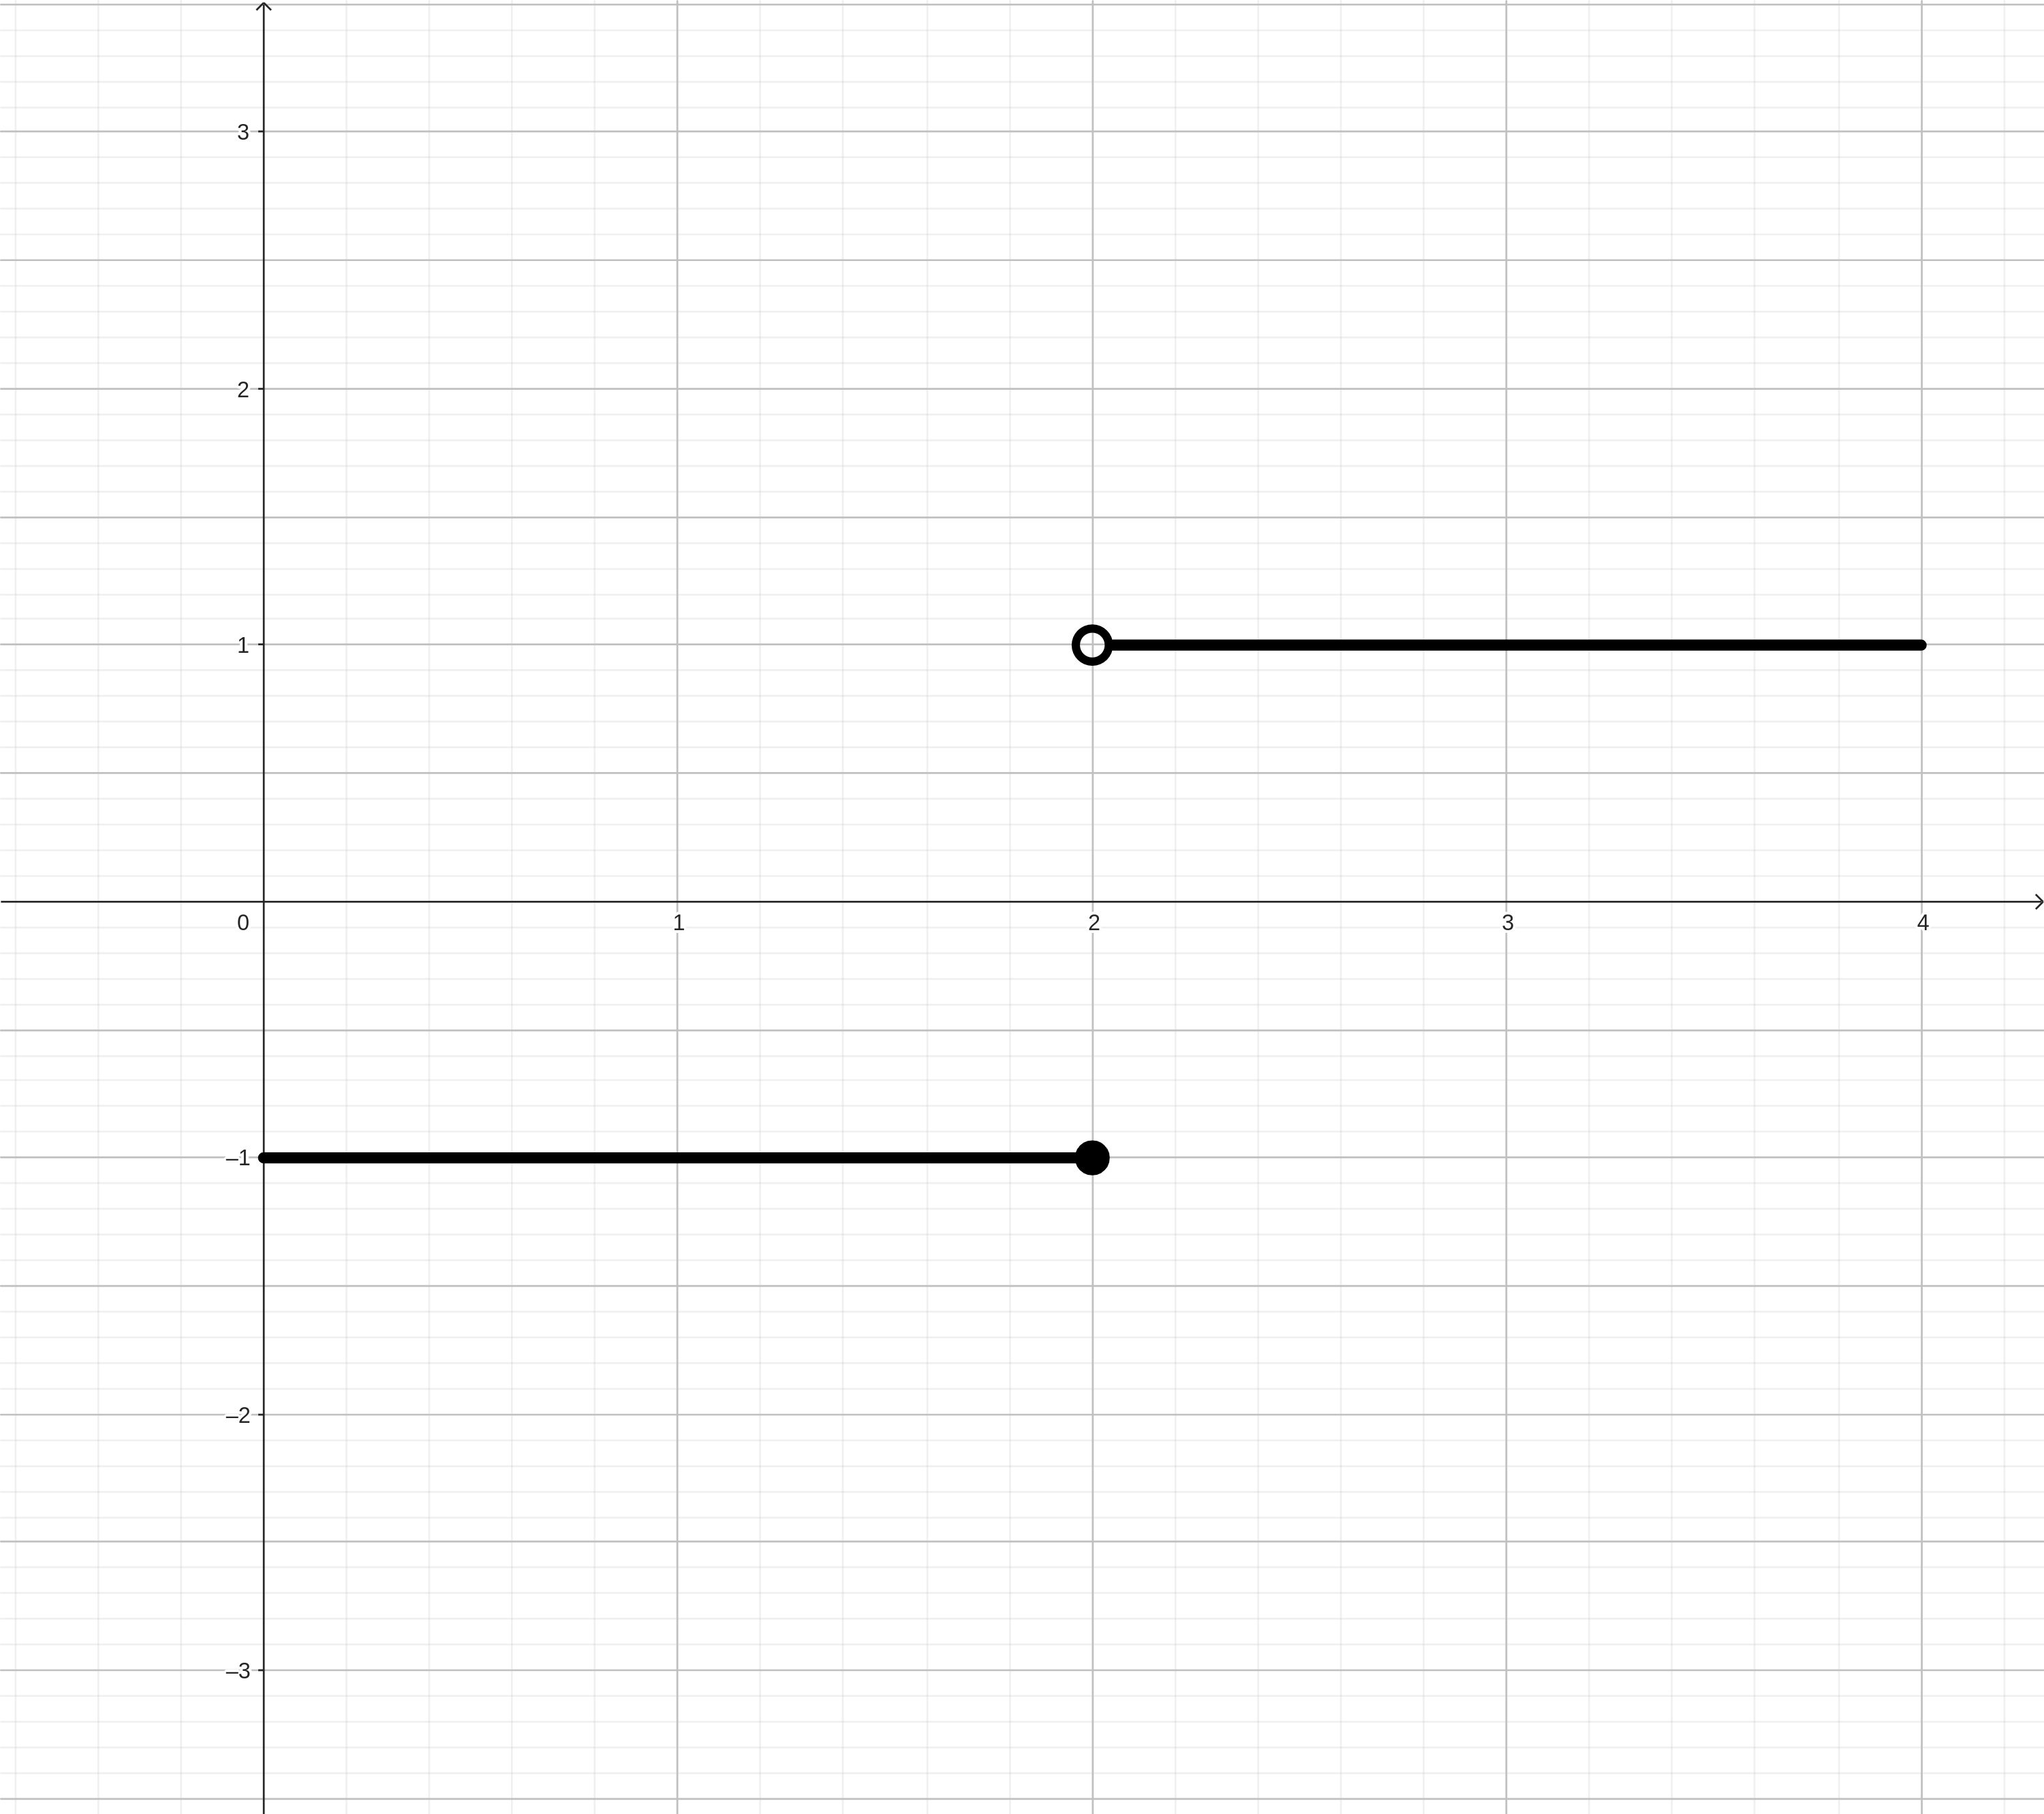
\includegraphics[width=300px]{../img/TeoremaZeriFunzioneNonContinua.png}
        \caption{Funzione definita a tratti per far vedere che la continuità nel teorema degli zeri è una condizione necessaria}
        \label{Figura_TeoraZeri}
    \end{figure}

    \item La seconda osservazione riguarda la quantità di punti in cui si può annullare la funzione. Come si legge dal teorema, il punto $c$ è garantito che esista ($\exists$) ma nessuno garantisce che è unico. Ci possono essere infatti un numero arbitrario di punti in cui la funzione si annulla, basti pensare al grafico delle funzioni goniometriche $\sin(x)$ e $\cos(x)$.
\end{itemize}


\pf{
  Questa dimostrazione a differenza delle altre è di tipo \textit{costruttivo}, cioè oltre a dimostrare il teorema fornisce un algoritmo di calcolo per trovare il punto $c$.\\

  Assumiamo $f(a) < 0$ e $f(b) > 0$. %Seguiamo una procedura iterativa che ci permetterà di costruire due successioni: $(a_n)_n$ e $(b_n)_n$ dove $a_1 = a$, $b_1 = b$, $\forall n, f(a_n) < 0$ e $\forall n, f(b_n) > 0$. 
  L'idea dietro questa dimostrazione è appunto trovare un algoritmo di calcolo che permetta di determinare il punto $c$. Avendo un punto $a$ in cui la funzione è \textbf{negativa} e un punto $b$ in cui la funzione è \textbf{positiva} ci deve essere un punto che giace tra $a$ e $b$ in cui la funzione si annulla. Per trovarlo andiamo a "tentativi" dividendo l'intervallo a metà con la formula:
  \begin{equation*}
    \dfrac{a+b}{2}
  \end{equation*}
  Da qui possiamo avere 3 casi:
  \begin{enumerate}
    \item $f\left(\dfrac{a + b}{2}\right) = 0$. In questo caso abbiamo trovato il punto $c$ proprio perché la funzione si annula. Quindi abbiamo finito!
      \begin{equation*}
        c = \dfrac{a+b}{2}
      \end{equation*}

      \item $f\left(\dfrac{a + b}{2}\right) < 0$. In questo caso non abbiamo trovato il punto $c$, ma bensì la funzione ci ha restituito un punto negativo. Essendo il punto $f(b)$ ancora maggiore di $0$ per ipotesi, possiamo applicare nuovamente questa procedura (cioè di suddividere l'intervallo a metà), però cambiando il punto $a$, in quanto adesso diventa:
      \begin{equation*}
        a_2 := \dfrac{a+b}{2}
      \end{equation*}

    \item $f\left(\dfrac{a + b}{2}\right) > 0$. L'idea di questo punto è identica a quella del punto 2, semplicemente invece che assegnare un valore diverso ad $a$, lo assegnamo a $b$ perché questa volta il valore della funzione è positivo invece che negativo.
      \begin{equation*}
        b_2 := \dfrac{a+b}{2}
      \end{equation*}
  \end{enumerate}
  Con i punti 2 e 3, riassegnando il valore ad $a$ o $b$, restringiamo l'intervallo su cui vogliamo applicare questo algoritmo per trovare il punto $c$. Ed essendo che ad ogni iterazione ci avviciniamo sempre di più, a forza di stringere l'intervallo prima o poi arriveremo a $c$.\\
  \textbf{Nota:} Ad ogni iterazione, se la funzione non si annulla, dobbiamo sostituire il valore del punto al corrispettivo punto $a$ o $b$ in modo che la funzione mantenga lo stesso segno. Questo perché se invertissimo i punti ci troveremmo in un caso in qui $f(a) > 0$ e $f(b) > 0$, cosa che ovviamente annullerebbe il teorema. Quindi nel caso del punto 2 in cui sostituiamo il nuovo punto ad $a$, lo facciamo soltanto perché per ipotesi $f(a) < 0$ e la funzione nel nuovo punto è negativa. Se per ipotesi avessimo scelto $f(a) > 0$ avremmo dovuto sostituire il nuovo punto in $b$, e vice versa.\\

  Essendo che dobbiamo ripete l'algoritmo, il caso \textit{n}-arrio diventa:
  \begin{enumerate}
    \item 
      \begin{equation*}
        f\left(\dfrac{a_n + b_n}{2}\right) = 0 \;\; \qquad \qquad \qquad \text{Fine:} \;\; \qquad \qquad \qquad c = \dfrac{a_n + b_n}{2}
      \end{equation*}

    \item 
      \begin{equation*}
        f\left(\dfrac{a_n + b_n}{2}\right) < 0 \qquad \text{Ieriamo nuovamente:} \qquad a_{n + 1}:= \dfrac{a_n + b_n}{2}
      \end{equation*}
      
    \item 
      \begin{equation*}
        f\left(\dfrac{a_n + b_n}{2}\right) > 0 \qquad \text{Ieriamo nuovamente:} \qquad b_{n + 1}:= \dfrac{a_n + b_n}{2}
      \end{equation*}

  \end{enumerate}

  Se l'algoritmo termina al passo $p \in \mathbb{N}$ significa che:
  \begin{equation*}
    f\left(\dfrac{a_p + b_p}{2}\right) = 0 \qquad \text{e quindi:} \qquad c = \dfrac{a_n + b_n}{2}
  \end{equation*}
  Altrimenti la procedura non termina: in quaso avremo costrutito due successioni $(a_n)_n$ e $(b_n)_n$ contenute in $[a, b]$. Scriviamo di seguito le proprietà di queste 2 successioni:
  \begin{enumerate}[label=\roman*.]
    \item $a_n \leq a_{n+1} \forall n \in \mathbb{N}$ \quad e \quad $b_n \leq b_{n+1} \forall n \in \mathbb{N}$

    \item $a_n \leq b_n \forall n \in \mathbb{N}$ 
      
    \item $f(a_n) < 0, \;\; f(b_n) > 0 \quad \forall n \in \mathbb{N}$
    
    \item 
      \begin{equation*}
        b_n - a_n = \dfrac{b_{n-1} - a_{n-1}}{2} \qquad \forall n
      \end{equation*}
      Se si espandono i vari passaggi si vede che in realtà ad ogni itarazione si divide l'intervallo iniziale $[a, b]$ in 2:
      \begin{equation*}
        b_n - a_n = \dfrac{b_{n-1} - a_{n-1}}{2} = \dfrac{b_{n-2} - a_{n-2}}{2^2} = \dfrac{b_{n-2} - a_{n-2}}{2^3}  = \cdots = \dfrac{b_1 - a_1}{2^{n-1}}
      \end{equation*}
  \end{enumerate}

  A questo punto vogliamo dimostrare che:
  \begin{equation*}
    \begin{cases*}
      \lim \limits_{n \to +\infty} a_n = \lim \limits_{n \to +\infty} b_n = c\\
      \\
      f(c) = 0
    \end{cases*}
  \end{equation*}
    Dal punto (i) e (ii) ricaviamo che sia $(a_n)_n$ sia $(b_n)_n$ sono \textbf{limitate}.
    \begin{equation*}
      (a_n)_n \subseteq [a, b] \implies a_n \nearrow \; \forall n \implies \exists \lim_{n \to +\infty} a_n = \alpha \in \mathbb{R}
    \end{equation*}
    \begin{equation*}
      (b_n)_n \subseteq [a, b] \implies b_n \nearrow \; \forall n \implies \exists \lim_{n \to +\infty} b_n = \beta \in \mathbb{R}
    \end{equation*}
    Dal punto (iv) e da quanto abbiamo ricavato possiamo fare il limite che tende a $+\infty$ di $b_n - a_n$:
    \begin{align*}
      \lim_{n \to +\infty} b_n - a_n &= \lim_{n \to +\infty} \dfrac{b_1 - a_1}{2^{n-1}}\\
      \beta - \alpha &= 0
    \end{align*}
    Quindi $\beta = \alpha$ e le due successioni hanno lo stesso limite! Abbiamo quindi provato che:
    \begin{equation*}
      \lim \limits_{n \to +\infty} a_n = \lim \limits_{n \to +\infty} b_n := c
    \end{equation*}
    Ci resta da dimostrare che $f(c) = 0$. Da quanto appena dimostrato e dal primo lemma di questa prova:
    \begin{equation*}
      \lim \limits_{n \to +\infty} f(a_n) = f(c)
    \end{equation*}
    Poiché $a_n \to c$. Inoltre dal punto (iii) sappiamo che $f(a_n) < 0 \; \forall n \in \mathbb{N}$. Usando il secondo lemma preliminare alla prova:
    \begin{equation*}
      f(c) \leq 0
    \end{equation*}
    Se facciamo lo stesso per $f(b_n)$:
    \begin{equation*}
      \lim \limits_{n \to +\infty} f(b_n) = f(c) \geq 0
    \end{equation*}
    Avendo contemporaneamente $f(c) \leq 0$ e $f(c) \geq 0$:
    \begin{equation*}
      f(c) = 0
    \end{equation*}
    \hfill Qed.
}

\subsection{Radici di un polinomio di grado dispari}

%AGGIUNGERE DIMOSRAZIONE 

\thm{
Ogni polinomio di grado dispari ha almeno un radice reale.
}
Corollario:
Tutti i polinomi di grado dispari assumono \textbf{tutti i valori reali}. Questo implica che una funzione che è definita tramite un polinomio di grado dispari è una funzione \textbf{suriettiva}, in quanto ha come immagine $\mathbb{R}$.\\

È facile ricordarsi questo teorema perché tutti i polinomi di grado dispari hanno il termine di grado maggiore (che in quanto dispari) è soggetto al segno dell'argomento del polinomio. Cioè $x^3$ avrà lo stesso segno di $x$, mentre questo non vale per i polinomi di grado pari in quanto $x^8$ avrà sempre segno positivo. Se quindi si fanno i limiti per $+\infty$ e $-\infty$ di un polinomio di grado dispari, da una parte andrà sempre a $+\infty$ e dall'altra andrà sempre a $-\infty$. Ed essendo i polinomi funzioni continue, sono costretti a toccare tutti i valori dell'asse delle ordinate almeno una volta. Inoltre, visto che da una parte hanno valori positivi, dall'altra negativi e sono continui, esiste per forza un punto in cui si annullano (dal teorema degli zeri) e sarà proprio lì la loro radice.

\subsection{Teorema di Weierstrass}
\subsubsection{Formulazione 1} %COSA ME NE FACCIO DI DUE FORMULAZIONE???

\dfn {
$f:A \to \mathbb{R}$
\begin{enumerate}
    \item $x_0 \in A: x_0$ si dice punto di \textbf{massimo assoluto} di $f$ se:
    \begin{equation*}
        f(x) \leq f(x_0) \quad \forall x \in A
    \end{equation*}
    
    \item $x_0 \in A: x_0$ si dice punto di \textbf{minimo assoluto} di $f$ se:
    \begin{equation*}
        f(x_0) \leq f(x) \quad \forall x \in A
    \end{equation*}
\end{enumerate}
}

\thm{
Una funzione continua, in un intervallo chiuso e limitato, ammette il massimo e il minimo assoluti della funzione.\\
$f: [a,b] \to \mathbb{R}$ continua, allora:
\begin{equation*}
    \exists x_0 \in [a,b]: f(x) \leq f(x_0) = \vcentcolon M \quad \forall x \in [a,b]
\end{equation*}
\begin{equation*}
    \exists x_1 \in [a,b]: f(x) \leq f(x_1) = \vcentcolon m \quad \forall x \in [a,b]
\end{equation*}
}
L'immagine di $f$ nell'intervallo $[a,b]$ corrisponderà a $[m, M]$.

\subsubsection{Formulazione 2} %SONO NECESSARIE DUE FORMULAZIONI?
\thm{
$f:[a,b]\to \mathbb{R}$ continua, allora:
\begin{equation*}
    \exists M = \max f([a,b])
\end{equation*}
\begin{equation*}
    \exists m = \min f([a,b])
\end{equation*}
}
